%%%%%%%%%%%%%%%%%%%%%%%%%%%%%%%%%%%%%%%%%
% University Assignment Title Page 
% LaTeX Template
% Version 1.0 (27/12/12)
%
% This template has been downloaded from:
% http://www.LaTeXTemplates.com
%
% Original author:
% WikiBooks (http://en.wikibooks.org/wiki/LaTeX/Title_Creation)
%
% License:
% CC BY-NC-SA 3.0 (http://creativecommons.org/licenses/by-nc-sa/3.0/)
% 
% Instructions for using this template:
% This title page is capable of being compiled as is. This is not useful for 
% including it in another document. To do this, you have two options: 
%
% 1) Copy/paste everything between \begin{document} and \end{document} 
% starting at \begin{titlepage} and paste this into another LaTeX file where you 
% want your title page.
% OR
% 2) Remove everything outside the \begin{titlepage} and \end{titlepage} and 
% move this file to the same directory as the LaTeX file you wish to add it to. 
% Then add %%%%%%%%%%%%%%%%%%%%%%%%%%%%%%%%%%%%%%%%%
% University Assignment Title Page 
% LaTeX Template
% Version 1.0 (27/12/12)
%
% This template has been downloaded from:
% http://www.LaTeXTemplates.com
%
% Original author:
% WikiBooks (http://en.wikibooks.org/wiki/LaTeX/Title_Creation)
%
% License:
% CC BY-NC-SA 3.0 (http://creativecommons.org/licenses/by-nc-sa/3.0/)
% 
% Instructions for using this template:
% This title page is capable of being compiled as is. This is not useful for 
% including it in another document. To do this, you have two options: 
%
% 1) Copy/paste everything between \begin{document} and \end{document} 
% starting at \begin{titlepage} and paste this into another LaTeX file where you 
% want your title page.
% OR
% 2) Remove everything outside the \begin{titlepage} and \end{titlepage} and 
% move this file to the same directory as the LaTeX file you wish to add it to. 
% Then add %%%%%%%%%%%%%%%%%%%%%%%%%%%%%%%%%%%%%%%%%
% University Assignment Title Page 
% LaTeX Template
% Version 1.0 (27/12/12)
%
% This template has been downloaded from:
% http://www.LaTeXTemplates.com
%
% Original author:
% WikiBooks (http://en.wikibooks.org/wiki/LaTeX/Title_Creation)
%
% License:
% CC BY-NC-SA 3.0 (http://creativecommons.org/licenses/by-nc-sa/3.0/)
% 
% Instructions for using this template:
% This title page is capable of being compiled as is. This is not useful for 
% including it in another document. To do this, you have two options: 
%
% 1) Copy/paste everything between \begin{document} and \end{document} 
% starting at \begin{titlepage} and paste this into another LaTeX file where you 
% want your title page.
% OR
% 2) Remove everything outside the \begin{titlepage} and \end{titlepage} and 
% move this file to the same directory as the LaTeX file you wish to add it to. 
% Then add %%%%%%%%%%%%%%%%%%%%%%%%%%%%%%%%%%%%%%%%%
% University Assignment Title Page 
% LaTeX Template
% Version 1.0 (27/12/12)
%
% This template has been downloaded from:
% http://www.LaTeXTemplates.com
%
% Original author:
% WikiBooks (http://en.wikibooks.org/wiki/LaTeX/Title_Creation)
%
% License:
% CC BY-NC-SA 3.0 (http://creativecommons.org/licenses/by-nc-sa/3.0/)
% 
% Instructions for using this template:
% This title page is capable of being compiled as is. This is not useful for 
% including it in another document. To do this, you have two options: 
%
% 1) Copy/paste everything between \begin{document} and \end{document} 
% starting at \begin{titlepage} and paste this into another LaTeX file where you 
% want your title page.
% OR
% 2) Remove everything outside the \begin{titlepage} and \end{titlepage} and 
% move this file to the same directory as the LaTeX file you wish to add it to. 
% Then add \input{./title_page_1.tex} to your LaTeX file where you want your
% title page.
%t
%%%%%%%%%%%%%%%%%%%%%%%%%%%%%%%%%%%%%%%%%
\title{Neo4j cơ bản và ứng dụng}
%----------------------------------------------------------------------------------------
%	PACKAGES AND OTHER DOCUMENT CONFIGURATIONS
%----------------------------------------------------------------------------------------

\documentclass[12pt]{article}
\usepackage[T5]{fontenc}
\usepackage[utf8]{inputenc}
\usepackage[vietnamese,english]{babel}
\usepackage{amsmath}
\usepackage{graphicx}
\usepackage[colorinlistoftodos]{todonotes}

\usepackage{hyperref}
\hypersetup{
    colorlinks=true,
    linkcolor=blue,
    filecolor=magenta,      
    urlcolor=cyan,
}


\begin{document}

\begin{titlepage}

\newcommand{\HRule}{\rule{\linewidth}{0.5mm}} % Defines a new command for the horizontal lines, change thickness here

\center % Center everything on the page
 
%----------------------------------------------------------------------------------------
%	HEADING SECTIONS
%----------------------------------------------------------------------------------------

\textsc{\LARGE Đại học Khoa học tự nhiên}\\[1.5cm] % Name of your university/college
\textsc{\Large Ngành hệ thống thông tin}\\[0.5cm] % Major heading such as course name
\textsc{\large Môn học: Cơ sở dữ liệu nâng cao}\\[0.5cm] % Minor heading such as course title

%----------------------------------------------------------------------------------------
%	TITLE SECTION
%----------------------------------------------------------------------------------------

\HRule \\[0.4cm]
{ \huge \bfseries Neo4j cơ bản và ứng dụng}\\[0.4cm] % Title of your document
\HRule \\[1.5cm]
 
%----------------------------------------------------------------------------------------
%	AUTHOR SECTION
%----------------------------------------------------------------------------------------

\begin{minipage}{0.4\textwidth}
\begin{flushleft} \large
\emph{Học viên:}\\
Thái Thiện -- 17C 12 031 % Your name
\end{flushleft}
\end{minipage}
~
\begin{minipage}{0.4\textwidth}
\begin{flushright} \large
\emph{Giảng viên:} \\
TS. Nguyễn Trần Minh Thư % Supervisor's Name
\end{flushright}
\end{minipage}\\[2cm]

% If you don't want a supervisor, uncomment the two lines below and remove the section above
%\Large \emph{Author:}\\
%John \textsc{Smith}\\[3cm] % Your name

%----------------------------------------------------------------------------------------
%	DATE SECTION
%----------------------------------------------------------------------------------------

% I don't want day because it is English
% {\large \today}\\[2cm] % Date, change the \today to a set date if you want to be precise

%----------------------------------------------------------------------------------------
%	LOGO SECTION
%----------------------------------------------------------------------------------------


\includegraphics{logo/rsz_3logo-khtn.png}\\[1cm] % Include a department/university logo - this will require the graphicx package
 
%----------------------------------------------------------------------------------------

\vfill % Fill the rest of the page with whitespace

\end{titlepage}


\section{Giới thiệu}
Neo4j là nền tảng cơ sở dữ liệu đồ thị (Neo4j Graph Platform) được công ty Neo4j phát triển. 

Trang chủ:  \url{https://neo4j.com}   
% \section{Some \LaTeX{} Examples}
% \label{sec:examples}

\subsection{Các phiên bản}
Neo4j có 2 phiên bản \footnote{\url{https://neo4j.com/subscriptions/}}

\begin{itemize}
\item \textbf{Community Edition} - Phiên bản cộng đồng: Đây là phiên bản miễn phí mã nguồn mở. Thích hợp cho các dự án nhỏ.
\item \textbf{Enterprise Edition} - Phiên bản doanh nghiệp: hiên bản có phí cho doanh nghiệp, có thêm nhiều chức năng như khả năng mở rộng theo chiều dài và chiều sâu, chức năng quản lý phân quyền. Ngoài ra, hiệu suất của phiên bản doanh nghiệp cao hơn phiên bản cộng đồng (vd: câu truy vấn nhanh hơn 70\%, ghi dữ liệu nhanh gấp 5 lần). Phiên bản doanh nghiệp bao gồm hỗ trợ kỹ thuật từ Neo4j 
\end{itemize}

\subsection{Cài đặt}
Tài về:  \url{https://neo4j.com/download/}  
Có thể cài bảng Neo4j Desktop trên máy tính cá nhân. 


\section{Cơ sở dữ liệu đồ thị}
Neo4j sử dụng Mô hình biểu đồ thuộc tính được gắn nhãn (Labeled Property Graph Mode). 

Mô hình bao gồm 4 thành phần: 

\begin{itemize}
\item Nút (nodes)
\item Quan hệ (relationships)
\item Thuộc tính  (properties)
\item Nhãn (labels)
\end{itemize}

\subsection{Nút (nodes)}
Nút (nodes) chứa các thuộc tính (properties). Một nút có thể xem là một bảng ghi gồm nhiều các cặp khóa - giá trị tùy ý. Trong Neo4j, khóa là chuổi còn giá trị là chuỗi Java và các kiểu dữ liệu nguyên thủy, và mảng của các dữ liệu đó. 

% % Commands to include a figure:
\begin{figure}[h]
\centering

\includegraphics[width=0.5\textwidth]{image/node.PNG}
\caption{\label{fig:node} Nút}
\end{figure}

\begin{figure}[h]
\centering
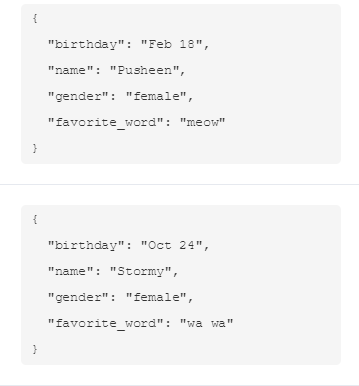
\includegraphics[width=0.5\textwidth]{image/thuoc_tinh.PNG}
\caption{\label{fig:node} Thuộc tính của nút}
\end{figure}

Mỗi nút có thể chứa 1 (hoặc nhiều) nhãn (labels). Nhãn giúp nhóm các nút lại với nhau. Có thể hiểu nhãn của nút là loại thực thể (mèo, đồ ăn, ...) của nút đó. Ví dụ hình \ref{fig:catfoodnode}, Nút xanh gán nhãn mèo, còn nút đỏ gán nhãn thức ăn.

\begin{figure}[h]
\centering
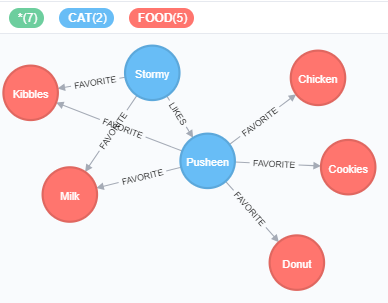
\includegraphics[width=0.5\textwidth]{image/complete_node_with_cat_and_food.PNG}
\caption{\label{fig:catfoodnode} Nút mèo và nút thức ăn}
\end{figure}

\subsection{Quan hệ (relationships)}
Quan hệ nối các nút lại để tạo thành biểu đồ. Mỗi quan hệ luôn có: 

\begin{itemize}
\item Tên quan hệ
\item Hướng 
\item Nút đầu
\item Nút cuối
\end{itemize}

Hình \ref{fig:relationships} biểu diễn quan hệ LIKES từ nút CAT có name = "Stormy" đến nút CAT có name = "Pusheen"

\begin{figure}[h]
\centering
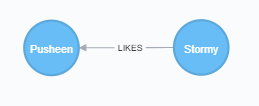
\includegraphics[width=0.5\textwidth]{image/relationships.PNG}
\caption{\label{fig:relationships} Quan hệ LIKES từ mèo Stormy đối với Pusheen}
\end{figure}

Quan hệ có thể chứa thuộc tính (properties) như nút (hình \ref{fig:relationshipsprop}). 

\begin{figure}[h]
\centering
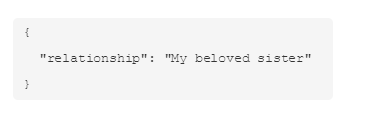
\includegraphics[width=0.5\textwidth]{image/quan_he_thuoc_tin.PNG}
\caption{\label{fig:relationshipsprop} Quan hệ LIKES từ mèo Stormy đối với Pusheen}
\end{figure}


\section{Cypher}



Comments can be added to the margins of the document using the \todo{Here's a comment in the margin!} todo command, as shown in the example on the right. You can also add inline comments too:

\todo[inline, color=green!40]{This is an inline comment.}

\subsection{Tables and Figures}

Use the table and tabular commands for basic tables --- see Table~\ref{tab:widgets}, for example. You can upload a figure (JPEG, PNG or PDF) using the files menu. To include it in your document, use the includegraphics command as in the code for Figure~\ref{fig:frog} below.

% % Commands to include a figure:
% \begin{figure}
% \centering
% 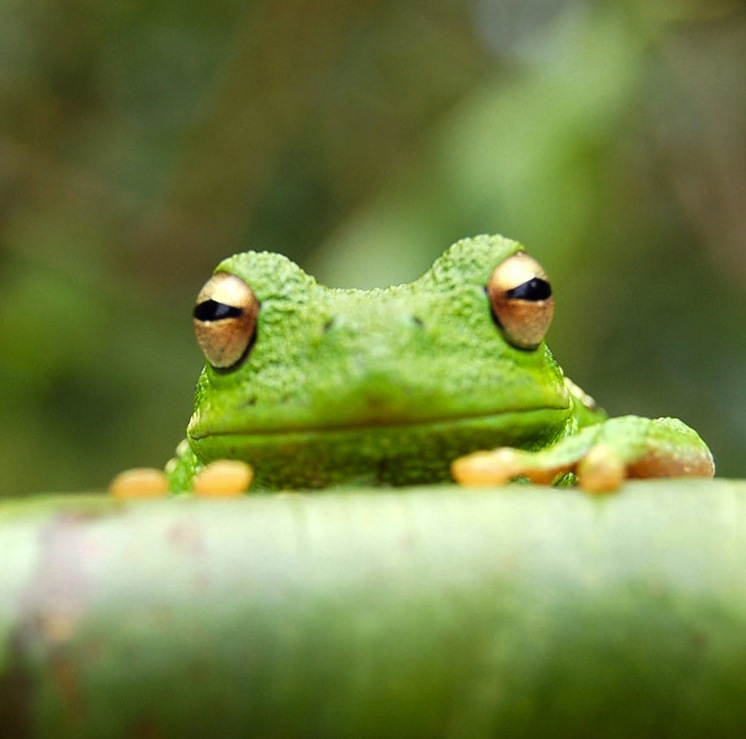
\includegraphics[width=0.5\textwidth]{frog.jpg}
% \caption{\label{fig:frog}This is a figure caption.}
% \end{figure}

% \begin{table}
% \centering
% \begin{tabular}{l|r}
% Item & Quantity \\\hline
% Widgets & 42 \\
% Gadgets & 13
% \end{tabular}
% \caption{\label{tab:widgets}An example table.}
% \end{table}

\subsection{Mathematics}

\LaTeX{} is great at typesetting mathematics. Let $X_1, X_2, \ldots, X_n$ be a sequence of independent and identically distributed random variables with $\text{E}[X_i] = \mu$ and $\text{Var}[X_i] = \sigma^2 < \infty$, and let
$$S_n = \frac{X_1 + X_2 + \cdots + X_n}{n}
      = \frac{1}{n}\sum_{i}^{n} X_i$$
denote their mean. Then as $n$ approaches infinity, the random variables $\sqrt{n}(S_n - \mu)$ converge in distribution to a normal $\mathcal{N}(0, \sigma^2)$.

\subsection{Lists}

You can make lists with automatic numbering \dots

\begin{enumerate}
\item Like this,
\item and like this.
\end{enumerate}
\dots or bullet points \dots
\begin{itemize}
\item Like this,
\item and like this.
\end{itemize}

We hope you find write\LaTeX\ useful, and please let us know if you have any feedback using the help menu above.

\end{document} to your LaTeX file where you want your
% title page.
%t
%%%%%%%%%%%%%%%%%%%%%%%%%%%%%%%%%%%%%%%%%
\title{Neo4j cơ bản và ứng dụng}
%----------------------------------------------------------------------------------------
%	PACKAGES AND OTHER DOCUMENT CONFIGURATIONS
%----------------------------------------------------------------------------------------

\documentclass[12pt]{article}
\usepackage[T5]{fontenc}
\usepackage[utf8]{inputenc}
\usepackage[vietnamese,english]{babel}
\usepackage{amsmath}
\usepackage{graphicx}
\usepackage[colorinlistoftodos]{todonotes}

\usepackage{hyperref}
\hypersetup{
    colorlinks=true,
    linkcolor=blue,
    filecolor=magenta,      
    urlcolor=cyan,
}


\begin{document}

\begin{titlepage}

\newcommand{\HRule}{\rule{\linewidth}{0.5mm}} % Defines a new command for the horizontal lines, change thickness here

\center % Center everything on the page
 
%----------------------------------------------------------------------------------------
%	HEADING SECTIONS
%----------------------------------------------------------------------------------------

\textsc{\LARGE Đại học Khoa học tự nhiên}\\[1.5cm] % Name of your university/college
\textsc{\Large Ngành hệ thống thông tin}\\[0.5cm] % Major heading such as course name
\textsc{\large Môn học: Cơ sở dữ liệu nâng cao}\\[0.5cm] % Minor heading such as course title

%----------------------------------------------------------------------------------------
%	TITLE SECTION
%----------------------------------------------------------------------------------------

\HRule \\[0.4cm]
{ \huge \bfseries Neo4j cơ bản và ứng dụng}\\[0.4cm] % Title of your document
\HRule \\[1.5cm]
 
%----------------------------------------------------------------------------------------
%	AUTHOR SECTION
%----------------------------------------------------------------------------------------

\begin{minipage}{0.4\textwidth}
\begin{flushleft} \large
\emph{Học viên:}\\
Thái Thiện -- 17C 12 031 % Your name
\end{flushleft}
\end{minipage}
~
\begin{minipage}{0.4\textwidth}
\begin{flushright} \large
\emph{Giảng viên:} \\
TS. Nguyễn Trần Minh Thư % Supervisor's Name
\end{flushright}
\end{minipage}\\[2cm]

% If you don't want a supervisor, uncomment the two lines below and remove the section above
%\Large \emph{Author:}\\
%John \textsc{Smith}\\[3cm] % Your name

%----------------------------------------------------------------------------------------
%	DATE SECTION
%----------------------------------------------------------------------------------------

% I don't want day because it is English
% {\large \today}\\[2cm] % Date, change the \today to a set date if you want to be precise

%----------------------------------------------------------------------------------------
%	LOGO SECTION
%----------------------------------------------------------------------------------------


\includegraphics{logo/rsz_3logo-khtn.png}\\[1cm] % Include a department/university logo - this will require the graphicx package
 
%----------------------------------------------------------------------------------------

\vfill % Fill the rest of the page with whitespace

\end{titlepage}


\section{Giới thiệu}
Neo4j là nền tảng cơ sở dữ liệu đồ thị (Neo4j Graph Platform) được công ty Neo4j phát triển. 

Trang chủ:  \url{https://neo4j.com}   
% \section{Some \LaTeX{} Examples}
% \label{sec:examples}

\subsection{Các phiên bản}
Neo4j có 2 phiên bản \footnote{\url{https://neo4j.com/subscriptions/}}

\begin{itemize}
\item \textbf{Community Edition} - Phiên bản cộng đồng: Đây là phiên bản miễn phí mã nguồn mở. Thích hợp cho các dự án nhỏ.
\item \textbf{Enterprise Edition} - Phiên bản doanh nghiệp: hiên bản có phí cho doanh nghiệp, có thêm nhiều chức năng như khả năng mở rộng theo chiều dài và chiều sâu, chức năng quản lý phân quyền. Ngoài ra, hiệu suất của phiên bản doanh nghiệp cao hơn phiên bản cộng đồng (vd: câu truy vấn nhanh hơn 70\%, ghi dữ liệu nhanh gấp 5 lần). Phiên bản doanh nghiệp bao gồm hỗ trợ kỹ thuật từ Neo4j 
\end{itemize}

\subsection{Cài đặt}
Tài về:  \url{https://neo4j.com/download/}  
Có thể cài bảng Neo4j Desktop trên máy tính cá nhân. 


\section{Cơ sở dữ liệu đồ thị}
Neo4j sử dụng Mô hình biểu đồ thuộc tính được gắn nhãn (Labeled Property Graph Mode). 

Mô hình bao gồm 4 thành phần: 

\begin{itemize}
\item Nút (nodes)
\item Quan hệ (relationships)
\item Thuộc tính  (properties)
\item Nhãn (labels)
\end{itemize}

\subsection{Nút (nodes)}
Nút (nodes) chứa các thuộc tính (properties). Một nút có thể xem là một bảng ghi gồm nhiều các cặp khóa - giá trị tùy ý. Trong Neo4j, khóa là chuổi còn giá trị là chuỗi Java và các kiểu dữ liệu nguyên thủy, và mảng của các dữ liệu đó. 

% % Commands to include a figure:
\begin{figure}[h]
\centering

\includegraphics[width=0.5\textwidth]{image/node.PNG}
\caption{\label{fig:node} Nút}
\end{figure}

\begin{figure}[h]
\centering
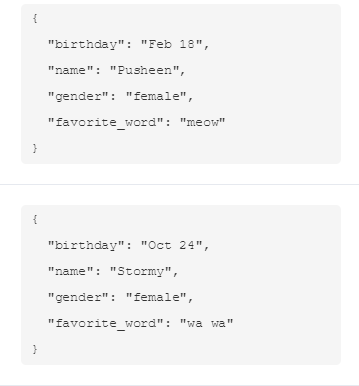
\includegraphics[width=0.5\textwidth]{image/thuoc_tinh.PNG}
\caption{\label{fig:node} Thuộc tính của nút}
\end{figure}

Mỗi nút có thể chứa 1 (hoặc nhiều) nhãn (labels). Nhãn giúp nhóm các nút lại với nhau. Có thể hiểu nhãn của nút là loại thực thể (mèo, đồ ăn, ...) của nút đó. Ví dụ hình \ref{fig:catfoodnode}, Nút xanh gán nhãn mèo, còn nút đỏ gán nhãn thức ăn.

\begin{figure}[h]
\centering
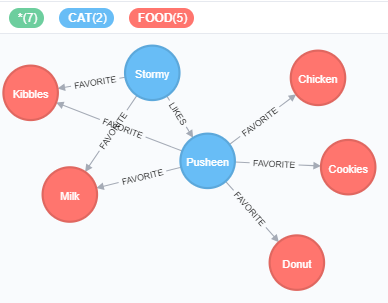
\includegraphics[width=0.5\textwidth]{image/complete_node_with_cat_and_food.PNG}
\caption{\label{fig:catfoodnode} Nút mèo và nút thức ăn}
\end{figure}

\subsection{Quan hệ (relationships)}
Quan hệ nối các nút lại để tạo thành biểu đồ. Mỗi quan hệ luôn có: 

\begin{itemize}
\item Tên quan hệ
\item Hướng 
\item Nút đầu
\item Nút cuối
\end{itemize}

Hình \ref{fig:relationships} biểu diễn quan hệ LIKES từ nút CAT có name = "Stormy" đến nút CAT có name = "Pusheen"

\begin{figure}[h]
\centering
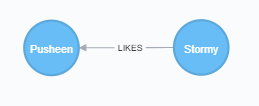
\includegraphics[width=0.5\textwidth]{image/relationships.PNG}
\caption{\label{fig:relationships} Quan hệ LIKES từ mèo Stormy đối với Pusheen}
\end{figure}

Quan hệ có thể chứa thuộc tính (properties) như nút (hình \ref{fig:relationshipsprop}). 

\begin{figure}[h]
\centering
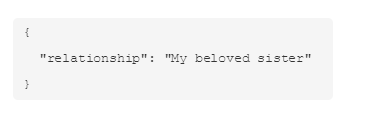
\includegraphics[width=0.5\textwidth]{image/quan_he_thuoc_tin.PNG}
\caption{\label{fig:relationshipsprop} Quan hệ LIKES từ mèo Stormy đối với Pusheen}
\end{figure}


\section{Cypher}



Comments can be added to the margins of the document using the \todo{Here's a comment in the margin!} todo command, as shown in the example on the right. You can also add inline comments too:

\todo[inline, color=green!40]{This is an inline comment.}

\subsection{Tables and Figures}

Use the table and tabular commands for basic tables --- see Table~\ref{tab:widgets}, for example. You can upload a figure (JPEG, PNG or PDF) using the files menu. To include it in your document, use the includegraphics command as in the code for Figure~\ref{fig:frog} below.

% % Commands to include a figure:
% \begin{figure}
% \centering
% 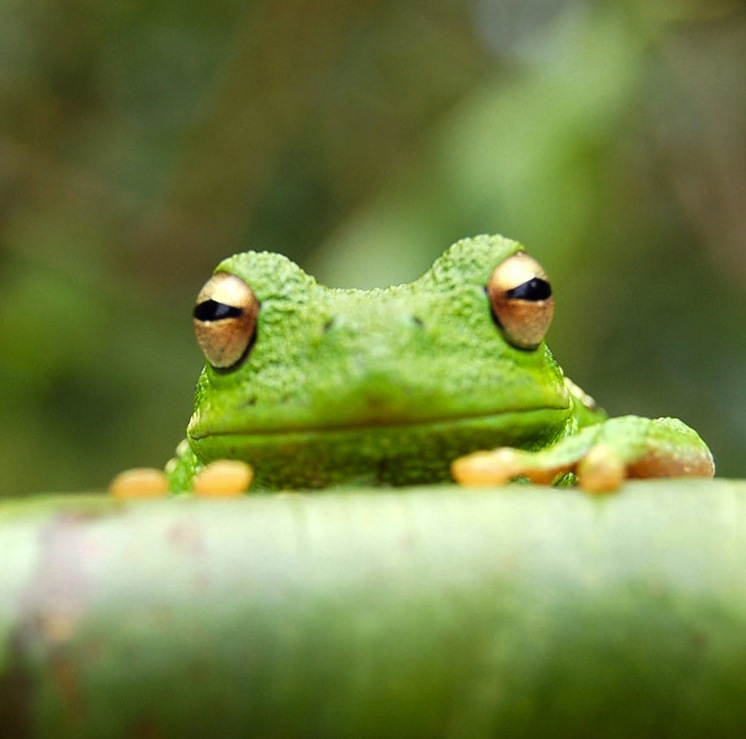
\includegraphics[width=0.5\textwidth]{frog.jpg}
% \caption{\label{fig:frog}This is a figure caption.}
% \end{figure}

% \begin{table}
% \centering
% \begin{tabular}{l|r}
% Item & Quantity \\\hline
% Widgets & 42 \\
% Gadgets & 13
% \end{tabular}
% \caption{\label{tab:widgets}An example table.}
% \end{table}

\subsection{Mathematics}

\LaTeX{} is great at typesetting mathematics. Let $X_1, X_2, \ldots, X_n$ be a sequence of independent and identically distributed random variables with $\text{E}[X_i] = \mu$ and $\text{Var}[X_i] = \sigma^2 < \infty$, and let
$$S_n = \frac{X_1 + X_2 + \cdots + X_n}{n}
      = \frac{1}{n}\sum_{i}^{n} X_i$$
denote their mean. Then as $n$ approaches infinity, the random variables $\sqrt{n}(S_n - \mu)$ converge in distribution to a normal $\mathcal{N}(0, \sigma^2)$.

\subsection{Lists}

You can make lists with automatic numbering \dots

\begin{enumerate}
\item Like this,
\item and like this.
\end{enumerate}
\dots or bullet points \dots
\begin{itemize}
\item Like this,
\item and like this.
\end{itemize}

We hope you find write\LaTeX\ useful, and please let us know if you have any feedback using the help menu above.

\end{document} to your LaTeX file where you want your
% title page.
%t
%%%%%%%%%%%%%%%%%%%%%%%%%%%%%%%%%%%%%%%%%
\title{Neo4j cơ bản và ứng dụng}
%----------------------------------------------------------------------------------------
%	PACKAGES AND OTHER DOCUMENT CONFIGURATIONS
%----------------------------------------------------------------------------------------

\documentclass[12pt]{article}
\usepackage[T5]{fontenc}
\usepackage[utf8]{inputenc}
\usepackage[vietnamese,english]{babel}
\usepackage{amsmath}
\usepackage{graphicx}
\usepackage[colorinlistoftodos]{todonotes}

\usepackage{hyperref}
\hypersetup{
    colorlinks=true,
    linkcolor=blue,
    filecolor=magenta,      
    urlcolor=cyan,
}


\begin{document}

\begin{titlepage}

\newcommand{\HRule}{\rule{\linewidth}{0.5mm}} % Defines a new command for the horizontal lines, change thickness here

\center % Center everything on the page
 
%----------------------------------------------------------------------------------------
%	HEADING SECTIONS
%----------------------------------------------------------------------------------------

\textsc{\LARGE Đại học Khoa học tự nhiên}\\[1.5cm] % Name of your university/college
\textsc{\Large Ngành hệ thống thông tin}\\[0.5cm] % Major heading such as course name
\textsc{\large Môn học: Cơ sở dữ liệu nâng cao}\\[0.5cm] % Minor heading such as course title

%----------------------------------------------------------------------------------------
%	TITLE SECTION
%----------------------------------------------------------------------------------------

\HRule \\[0.4cm]
{ \huge \bfseries Neo4j cơ bản và ứng dụng}\\[0.4cm] % Title of your document
\HRule \\[1.5cm]
 
%----------------------------------------------------------------------------------------
%	AUTHOR SECTION
%----------------------------------------------------------------------------------------

\begin{minipage}{0.4\textwidth}
\begin{flushleft} \large
\emph{Học viên:}\\
Thái Thiện -- 17C 12 031 % Your name
\end{flushleft}
\end{minipage}
~
\begin{minipage}{0.4\textwidth}
\begin{flushright} \large
\emph{Giảng viên:} \\
TS. Nguyễn Trần Minh Thư % Supervisor's Name
\end{flushright}
\end{minipage}\\[2cm]

% If you don't want a supervisor, uncomment the two lines below and remove the section above
%\Large \emph{Author:}\\
%John \textsc{Smith}\\[3cm] % Your name

%----------------------------------------------------------------------------------------
%	DATE SECTION
%----------------------------------------------------------------------------------------

% I don't want day because it is English
% {\large \today}\\[2cm] % Date, change the \today to a set date if you want to be precise

%----------------------------------------------------------------------------------------
%	LOGO SECTION
%----------------------------------------------------------------------------------------


\includegraphics{logo/rsz_3logo-khtn.png}\\[1cm] % Include a department/university logo - this will require the graphicx package
 
%----------------------------------------------------------------------------------------

\vfill % Fill the rest of the page with whitespace

\end{titlepage}


\section{Giới thiệu}
Neo4j là nền tảng cơ sở dữ liệu đồ thị (Neo4j Graph Platform) được công ty Neo4j phát triển. 

Trang chủ:  \url{https://neo4j.com}   
% \section{Some \LaTeX{} Examples}
% \label{sec:examples}

\subsection{Các phiên bản}
Neo4j có 2 phiên bản \footnote{\url{https://neo4j.com/subscriptions/}}

\begin{itemize}
\item \textbf{Community Edition} - Phiên bản cộng đồng: Đây là phiên bản miễn phí mã nguồn mở. Thích hợp cho các dự án nhỏ.
\item \textbf{Enterprise Edition} - Phiên bản doanh nghiệp: hiên bản có phí cho doanh nghiệp, có thêm nhiều chức năng như khả năng mở rộng theo chiều dài và chiều sâu, chức năng quản lý phân quyền. Ngoài ra, hiệu suất của phiên bản doanh nghiệp cao hơn phiên bản cộng đồng (vd: câu truy vấn nhanh hơn 70\%, ghi dữ liệu nhanh gấp 5 lần). Phiên bản doanh nghiệp bao gồm hỗ trợ kỹ thuật từ Neo4j 
\end{itemize}

\subsection{Cài đặt}
Tài về:  \url{https://neo4j.com/download/}  
Có thể cài bảng Neo4j Desktop trên máy tính cá nhân. 


\section{Cơ sở dữ liệu đồ thị}
Neo4j sử dụng Mô hình biểu đồ thuộc tính được gắn nhãn (Labeled Property Graph Mode). 

Mô hình bao gồm 4 thành phần: 

\begin{itemize}
\item Nút (nodes)
\item Quan hệ (relationships)
\item Thuộc tính  (properties)
\item Nhãn (labels)
\end{itemize}

\subsection{Nút (nodes)}
Nút (nodes) chứa các thuộc tính (properties). Một nút có thể xem là một bảng ghi gồm nhiều các cặp khóa - giá trị tùy ý. Trong Neo4j, khóa là chuổi còn giá trị là chuỗi Java và các kiểu dữ liệu nguyên thủy, và mảng của các dữ liệu đó. 

% % Commands to include a figure:
\begin{figure}[h]
\centering

\includegraphics[width=0.5\textwidth]{image/node.PNG}
\caption{\label{fig:node} Nút}
\end{figure}

\begin{figure}[h]
\centering
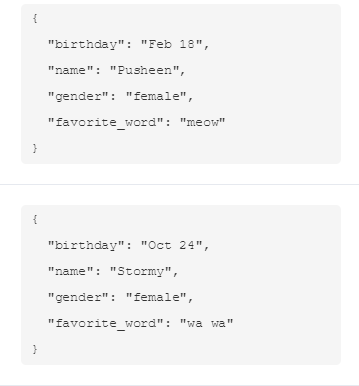
\includegraphics[width=0.5\textwidth]{image/thuoc_tinh.PNG}
\caption{\label{fig:node} Thuộc tính của nút}
\end{figure}

Mỗi nút có thể chứa 1 (hoặc nhiều) nhãn (labels). Nhãn giúp nhóm các nút lại với nhau. Có thể hiểu nhãn của nút là loại thực thể (mèo, đồ ăn, ...) của nút đó. Ví dụ hình \ref{fig:catfoodnode}, Nút xanh gán nhãn mèo, còn nút đỏ gán nhãn thức ăn.

\begin{figure}[h]
\centering
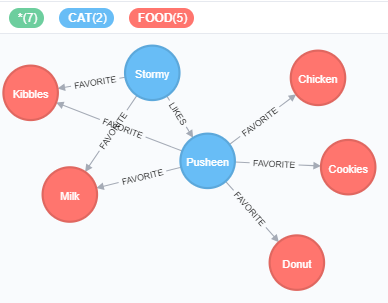
\includegraphics[width=0.5\textwidth]{image/complete_node_with_cat_and_food.PNG}
\caption{\label{fig:catfoodnode} Nút mèo và nút thức ăn}
\end{figure}

\subsection{Quan hệ (relationships)}
Quan hệ nối các nút lại để tạo thành biểu đồ. Mỗi quan hệ luôn có: 

\begin{itemize}
\item Tên quan hệ
\item Hướng 
\item Nút đầu
\item Nút cuối
\end{itemize}

Hình \ref{fig:relationships} biểu diễn quan hệ LIKES từ nút CAT có name = "Stormy" đến nút CAT có name = "Pusheen"

\begin{figure}[h]
\centering
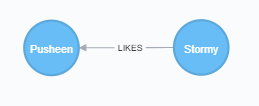
\includegraphics[width=0.5\textwidth]{image/relationships.PNG}
\caption{\label{fig:relationships} Quan hệ LIKES từ mèo Stormy đối với Pusheen}
\end{figure}

Quan hệ có thể chứa thuộc tính (properties) như nút (hình \ref{fig:relationshipsprop}). 

\begin{figure}[h]
\centering
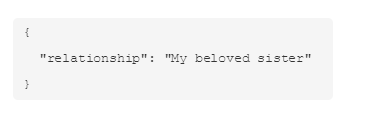
\includegraphics[width=0.5\textwidth]{image/quan_he_thuoc_tin.PNG}
\caption{\label{fig:relationshipsprop} Quan hệ LIKES từ mèo Stormy đối với Pusheen}
\end{figure}


\section{Cypher}



Comments can be added to the margins of the document using the \todo{Here's a comment in the margin!} todo command, as shown in the example on the right. You can also add inline comments too:

\todo[inline, color=green!40]{This is an inline comment.}

\subsection{Tables and Figures}

Use the table and tabular commands for basic tables --- see Table~\ref{tab:widgets}, for example. You can upload a figure (JPEG, PNG or PDF) using the files menu. To include it in your document, use the includegraphics command as in the code for Figure~\ref{fig:frog} below.

% % Commands to include a figure:
% \begin{figure}
% \centering
% 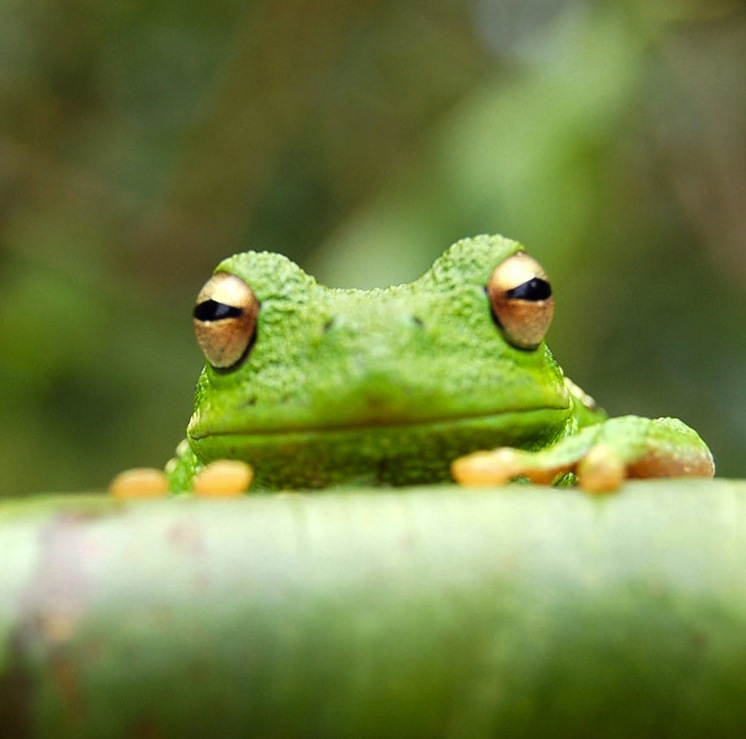
\includegraphics[width=0.5\textwidth]{frog.jpg}
% \caption{\label{fig:frog}This is a figure caption.}
% \end{figure}

% \begin{table}
% \centering
% \begin{tabular}{l|r}
% Item & Quantity \\\hline
% Widgets & 42 \\
% Gadgets & 13
% \end{tabular}
% \caption{\label{tab:widgets}An example table.}
% \end{table}

\subsection{Mathematics}

\LaTeX{} is great at typesetting mathematics. Let $X_1, X_2, \ldots, X_n$ be a sequence of independent and identically distributed random variables with $\text{E}[X_i] = \mu$ and $\text{Var}[X_i] = \sigma^2 < \infty$, and let
$$S_n = \frac{X_1 + X_2 + \cdots + X_n}{n}
      = \frac{1}{n}\sum_{i}^{n} X_i$$
denote their mean. Then as $n$ approaches infinity, the random variables $\sqrt{n}(S_n - \mu)$ converge in distribution to a normal $\mathcal{N}(0, \sigma^2)$.

\subsection{Lists}

You can make lists with automatic numbering \dots

\begin{enumerate}
\item Like this,
\item and like this.
\end{enumerate}
\dots or bullet points \dots
\begin{itemize}
\item Like this,
\item and like this.
\end{itemize}

We hope you find write\LaTeX\ useful, and please let us know if you have any feedback using the help menu above.

\end{document} to your LaTeX file where you want your
% title page.
%
%%%%%%%%%%%%%%%%%%%%%%%%%%%%%%%%%%%%%%%%%
%\title{Title page with logo}
%----------------------------------------------------------------------------------------
%	PACKAGES AND OTHER DOCUMENT CONFIGURATIONS
%----------------------------------------------------------------------------------------

\documentclass[12pt]{article}
\usepackage[english]{babel}
\usepackage[utf8x]{inputenc}
\usepackage{amsmath}
\usepackage{graphicx}
\usepackage[colorinlistoftodos]{todonotes}

\begin{document}

\begin{titlepage}

\newcommand{\HRule}{\rule{\linewidth}{0.5mm}} % Defines a new command for the horizontal lines, change thickness here

\center % Center everything on the page
 
%----------------------------------------------------------------------------------------
%	HEADING SECTIONS
%----------------------------------------------------------------------------------------

\textsc{\LARGE University Name}\\[1.5cm] % Name of your university/college
\textsc{\Large Major Heading}\\[0.5cm] % Major heading such as course name
\textsc{\large Minor Heading}\\[0.5cm] % Minor heading such as course title

%----------------------------------------------------------------------------------------
%	TITLE SECTION
%----------------------------------------------------------------------------------------

\HRule \\[0.4cm]
{ \huge \bfseries Title}\\[0.4cm] % Title of your document
\HRule \\[1.5cm]
 
%----------------------------------------------------------------------------------------
%	AUTHOR SECTION
%----------------------------------------------------------------------------------------

\begin{minipage}{0.4\textwidth}
\begin{flushleft} \large
\emph{Author:}\\
John \textsc{Smith} % Your name
\end{flushleft}
\end{minipage}
~
\begin{minipage}{0.4\textwidth}
\begin{flushright} \large
\emph{Supervisor:} \\
Dr. James \textsc{Smith} % Supervisor's Name
\end{flushright}
\end{minipage}\\[2cm]

% If you don't want a supervisor, uncomment the two lines below and remove the section above
%\Large \emph{Author:}\\
%John \textsc{Smith}\\[3cm] % Your name

%----------------------------------------------------------------------------------------
%	DATE SECTION
%----------------------------------------------------------------------------------------

{\large \today}\\[2cm] % Date, change the \today to a set date if you want to be precise

%----------------------------------------------------------------------------------------
%	LOGO SECTION
%----------------------------------------------------------------------------------------


\includegraphics{logo.png}\\[1cm] % Include a department/university logo - this will require the graphicx package
 
%----------------------------------------------------------------------------------------

\vfill % Fill the rest of the page with whitespace

\end{titlepage}


\begin{abstract}
Your abstract.
\end{abstract}

\section{Introduction}

Your introduction goes here! Some examples of commonly used commands and features are listed below, to help you get started.

If you have a question, please use the support box in the bottom right of the screen to get in touch. 

\section{Some \LaTeX{} Examples}
\label{sec:examples}

\subsection{Sections}

Use section and subsection commands to organize your document. \LaTeX{} handles all the formatting and numbering automatically. Use ref and label commands for cross-references.

\subsection{Comments}

Comments can be added to the margins of the document using the \todo{Here's a comment in the margin!} todo command, as shown in the example on the right. You can also add inline comments too:

\todo[inline, color=green!40]{This is an inline comment.}

\subsection{Tables and Figures}

Use the table and tabular commands for basic tables --- see Table~\ref{tab:widgets}, for example. You can upload a figure (JPEG, PNG or PDF) using the files menu. To include it in your document, use the includegraphics command as in the code for Figure~\ref{fig:frog} below.

% Commands to include a figure:
\begin{figure}
\centering
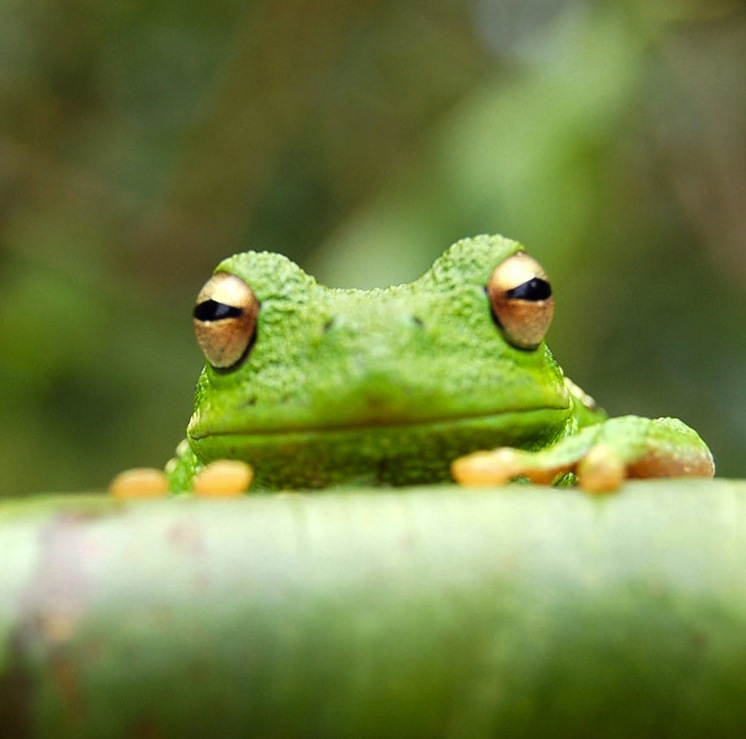
\includegraphics[width=0.5\textwidth]{frog.jpg}
\caption{\label{fig:frog}This is a figure caption.}
\end{figure}

\begin{table}
\centering
\begin{tabular}{l|r}
Item & Quantity \\\hline
Widgets & 42 \\
Gadgets & 13
\end{tabular}
\caption{\label{tab:widgets}An example table.}
\end{table}

\subsection{Mathematics}

\LaTeX{} is great at typesetting mathematics. Let $X_1, X_2, \ldots, X_n$ be a sequence of independent and identically distributed random variables with $\text{E}[X_i] = \mu$ and $\text{Var}[X_i] = \sigma^2 < \infty$, and let
$$S_n = \frac{X_1 + X_2 + \cdots + X_n}{n}
      = \frac{1}{n}\sum_{i}^{n} X_i$$
denote their mean. Then as $n$ approaches infinity, the random variables $\sqrt{n}(S_n - \mu)$ converge in distribution to a normal $\mathcal{N}(0, \sigma^2)$.

\subsection{Lists}

You can make lists with automatic numbering \dots

\begin{enumerate}
\item Like this,
\item and like this.
\end{enumerate}
\dots or bullet points \dots
\begin{itemize}
\item Like this,
\item and like this.
\end{itemize}

We hope you find write\LaTeX\ useful, and please let us know if you have any feedback using the help menu above.

\end{document}